% Independent reader R1, scan 007 only. Ink decisions, not mathematical emendations.
% Cursive alphabet conventions remain provisional at the first occurrence.
\scanpage{7}\mspage{6}
\deleted{$\mathrm{At}_{M}\,4:\ \forall X\in\unsure{M|\mathcal M},\ \Phi\in\widetilde{\unsure{\mathscr F|\mathcal F}}$, posant $\Phi^{X}=\{Y\in\Phi\mid X\ll Y\}$, $\Phi^{X}$ a un plus petit \unsure{élément}}

\margin{J'ai exprimé $\uline{\mathrm{At}}\,\deleted{\unsure{6}}5$ sans référence à $\mathscr F$ ou à $\widetilde{\mathscr F}$, mais directement en \unsure{termes|terme} de $(M,\leq,\ll,\mathrel{\tikz[baseline=-.4ex,x=.65em,y=.65em]{\draw (0,1.1)--(1,.5)--(0,-.1) (1,1.1)--(0,.5)--(1,-.1);}})$ $\nearrow$}%
$\mathrm{At}_{M}\,4$ \quad a) \deleted{Posant $X\ll Y\ \unsure{\Longleftrightarrow|\Longrightarrow}\ \unsure{Y|X}$ \unsure{contient}} \deleted{$\forall X,Y\in M,\ X\ll$ \unsure{défini}} \deleted{\unsure{est|ent} \unsure{minimal|minimum}} Si $X\ll Y$, alors il y a un \deleted{plus petit élément} \inserted{élément minimal} \inserted{dans} $\widetilde Y^{X}=\{Z\in\widetilde Y\mid X\ll Z\}$ \deleted{\unsure{i.e.} $X\ll Y'\leq Y\Longrightarrow Y'=Y$} \inserted{(posons $X\overset{\circ}{\ll}Y$ si c'est $Y$)}

\[
\begin{aligned}
\text{b) Alors}\quad & X\overset{\circ}{\ll}Y,\quad X\overset{\circ}{\ll}Y',\quad Y\mathrel{\tikz[baseline=-.4ex,x=.65em,y=.65em]{\draw (0,1.1)--(1,.5)--(0,-.1) (1,1.1)--(0,.5)--(1,-.1);}}Y'\ \Longrightarrow\ Y=Y'\\
\mathrm{At}_{M}\,\deleted{\unsure{5}}6\quad &\text{Si }X\mathrel{\tikz[baseline=-.4ex,x=.65em,y=.65em]{\draw (0,1.1)--(1,.5)--(0,-.1) (1,1.1)--(0,.5)--(1,-.1);}}Y,\ \text{alors }\ X\ll Y\ \Longrightarrow\ X\leq Y\\
\mathrm{At}_{M}\,\deleted{\unsure{6}}5\quad &X\overset{\circ}{\ll}Y\overset{\circ}{\ll}Z\ \Longrightarrow\ X\overset{\circ}{\ll}Z
\end{aligned}
\]
\margin{\tikz[x=.6em,y=.6em]{\draw (.95,0)..controls(-.3,-.15)and(-.2,1)..(.95,1.25); \draw[->] (.2,.95)..controls(-.18,1.15)and(0,2)..(.08,2.3)--(1.45,3);}}%

D'autre part, pour des $\mathscr F$ à figures de type fini, on peut laisser tomber l'élément de structure $\unsure{\widetilde{\mathscr F}|\mathscr F}$, \inserted{au profit de $\mathrel{\tikz[baseline=-.4ex,x=.65em,y=.65em]{\draw (0,1.1)--(1,.5)--(0,-.1) (1,1.1)--(0,.5)--(1,-.1);}}$,} et remplacer $\mathrm{At}_{M}\,1$ ; $\mathrm{At}_{M}\,3$ par (a) de la \deleted{$\mathrm{At}_{M}\,1\,(\mathrm{tf})$ Toute partie fermée majorée de $M$ est de t.f.} \deleted{At} page 5 (Toute partie fermée majorée de $M$ est de t.f.) et la condition b sur $ {\mathrel{\tikz[baseline=-.4ex,x=.65em,y=.65em]{\draw (0,1.1)--(1,.5)--(0,-.1) (1,1.1)--(0,.5)--(1,-.1);}}}^{*}$. (page 5)
% slanted
\margin{i.e. $X\mathrel{\tikz[baseline=-.4ex,x=.65em,y=.65em]{\draw (0,1.1)--(1,.5)--(0,-.1) (1,1.1)--(0,.5)--(1,-.1);}}Y$ et $X'\leq X,\ Y'\leq Y$ $\mathrel{\tikz[baseline=-.15ex,x=.5em,y=.28em]{\draw (0,.08)--(1.2,.08) (0,.42)--(1.2,.42) .. controls (1.42,.42) and (1.48,.15) .. (1.32,.12);}}X'\mathrel{\tikz[baseline=-.4ex,x=.65em,y=.65em]{\draw (0,1.1)--(1,.5)--(0,-.1) (1,1.1)--(0,.5)--(1,-.1);}}Y'$}%

Dans le cas général, quand on a simplement $\mathrel{\tikz[baseline=-.4ex,x=.65em,y=.65em]{\draw (0,1.1)--(1,.5)--(0,-.1) (1,1.1)--(0,.5)--(1,-.1);}}$ satisfaisant cette condition b) plus les conditions $\mathrm{At}_{M}\,4,5,6$, on trouve
% The added Phi de t.f. sits above the far-right de M,leq.
% The two curved strokes are reproduced as geometry, without assigning a
% parenthesis or an additional logical relation to either one.
\figure{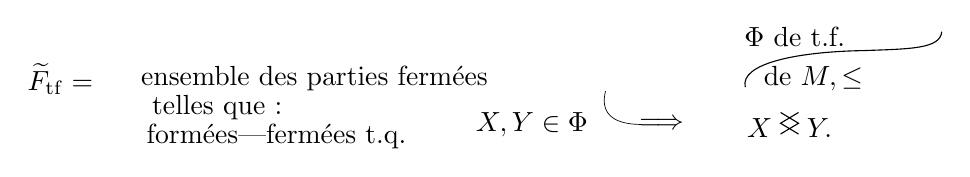
\begin{tikzpicture}[x=1em,y=1em,baseline=(current bounding box.center),every node/.style={inner sep=0pt}]
  \node[anchor=west] at (0,0) {$\widetilde{\mathscr F}_{\mathrm{tf}}=$};
  \node[anchor=west] at (4.1,0) {ensemble des parties fermées};
  \node[anchor=west] at (25.9,1.5) {\inserted{$\Phi$ de t.f.}};
  \node[anchor=west] at (26.6,0) {de $M,\leq$};
  \draw (25.95,-.3)..controls(25.75,.55)and(27.8,.98)..(30.25,1.02)
        ..controls(31.9,1.08)and(33,1.08)..(33.05,1.7);
  \node[anchor=west] at (4.3,-2.1) {\deleted{\unsure{formées|fermées} t.q.}};
  \node[anchor=west] at (4.5,-1.05) {\inserted{telles que :}};
  \node[anchor=west] at (16.2,-1.65) {$X,Y\in\Phi$};
  \node[anchor=west] at (22.1,-1.65) {$\Longrightarrow$};
  \node[anchor=west] at (26,-1.65) {$X\mathrel{\tikz[baseline=-.4ex,x=.65em,y=.65em]{\draw (0,1.1)--(1,.5)--(0,-.1) (1,1.1)--(0,.5)--(1,-.1);}}Y.$};
  % Thin return below the long f-stroke of fermées, toward the implication.
  \draw[line width=.25pt] (20.9,-.45)..controls(20.72,-1.15)and(21.05,-1.65)..(22.2,-1.65);
\end{tikzpicture}}

Pour avoir $\widetilde{\mathscr F}$, il faut cependant un choix de structure en plus : se donner certains antifiltres infinis dans l'ens ordonné $\widetilde{\mathscr F}_{\mathrm{tf}}$ précédent\ldots

On peut aussi interpréter $\mathscr F$ en termes de
\[
\begin{aligned}
\mathscr F^{*}&=\{\mathrm{Mulomb}(F)\mid F\in\mathscr F\}\subset\mathrm{Fig}(M)\\
\text{\unsure{\deleted{où}|où}}\quad\mathrm{Mulomb}(\unsure{F|\mathscr F})&=\{\deleted{\unsure{x|X}}\ \mathrm{Omb}(x)\mid X\in\widetilde F\}\\
\mathrm{Omb}\,X&=\{Y\in M\mid Y\ll X\}=M_{\ll x}.
\end{aligned}
\]
(cf Scholie GF p. 28, et axiomes, ou mieux à la \uline{page 32}), comme sous-atelier (pas néc. \unsure{spacieux|specieux}) de $\mathrm{Fig}(M)$.
